% !TEX root = ../Dissertation.tex

\chapter{NExUME: Adaptive Training and Inference for Deep Neural Networks under Intermittent Power Environments} \label{ch:nexume}

\section{Introduction}
\label{sec:nexume_intro}

Building upon the distributed inference systems presented in Chapter~\ref{ch:intelligent-inference}, this chapter addresses a fundamental challenge in deploying deep neural networks (DNNs) on energy harvesting platforms: the inherent mismatch between conventional DNN training paradigms and the intermittent nature of harvested power. While the Origin and Seeker frameworks from the previous chapter demonstrated how to optimize inference distribution and communication in energy harvesting wireless sensor networks (EH-WSNs), they assumed that individual nodes could execute their assigned DNN models when sufficient energy was available. However, this assumption overlooks a critical aspect: DNNs are typically trained for stable resource environments and fail to adapt to the variable and intermittent resource availability characteristic of energy harvesting systems.

The increasing demand for ubiquitous, sustainable, and energy-efficient computing, combined with advancements in energy harvesting systems, has spurred significant research into battery-less devices~\cite{intelligencebeyondedge, mouse, origin, wisp, MIT}. Such platforms represent the future of the Internet of Things (IoT) and energy harvesting wireless sensor networks. Equipped with modern machine learning techniques, these devices can revolutionize computing, monitoring, and analytics in remote, risky, and critical environments such as oil wells, mines, deep forests, oceans, remote industries, and smart cities. However, the intermittent and limited energy income of these deployments demands optimizations for ML applications at multiple levels, including the algorithm~\cite{eap, tianyi, intermittentNAS}, orchestration~\cite{chinchilla, origin}, compilation~\cite{alpaca}, and hardware development~\cite{resirca, islam2022enabling, usas} layers.

Despite these advancements, achieving consistent and accurate inference---thereby meeting service level objectives (SLOs)---in such intermittent environments remains a significant challenge, exacerbated by unpredictable resources, form-factor limitations, and variable computational availability, particularly when employing task-optimized deep neural networks.

\subsection{The Challenge of Intermittent Power}

Two major problems arise when performing DNN inference under intermittent power. First, energy variability presents a fundamental challenge. Even though DNNs can be tailored to match the average energy income of the energy harvesting source through pruning, quantization, distillation, or network architecture search (NAS)~\cite{netadapt, eap, intermittentNAS}, there is no guarantee that the energy income consistently meets or exceeds this average. When the income falls below the threshold, the system must halt the inference and checkpoint the intermediate states (via software or persistent hardware)~\cite{chinchilla, resirca}, resuming upon energy recovery. Depending on the EH profile, this might lead to significant delays and SLO violations.

Second, computational approximation becomes necessary to maintain continuous operation. EH-WSNs may skip some computations during energy shortfalls by dropping neurons (zero padding) or by approximating computations (quantization). Adding further approximation to save energy atop an already heavily reduced network can propagate errors through the layers, leading to significant accuracy drops~\cite{Zygarde, moreisless, DFI, kang}, further violating SLOs.

In certain energy-critical scenarios, even EH-WSNs applying state-of-the-art techniques fail to consistently meet SLOs, sometimes skipping entire inferences to deliver results on time. Fundamentally, while current DNNs can be trained or fine-tuned to fit within a given resource budget---be it compute, memory, or energy---they are not trained to expect a variable or intermittent resource income. Although intermittency-aware NAS~\cite{intermittentNAS} could alleviate certain problems, they often assume fixed resource constraints and do not account for real-time energy fluctuations.

Moreover, existing works like Keep in Balance~\cite{yen2023keep}, Stateful Neural Networks~\cite{yen2022stateful}, ePerceptive~\cite{patel2019eperceptive}, and Zygarde~\cite{Zygarde} address aspects of intermittent computing but do not integrate energy variability awareness directly into the training and inference processes to enable dynamic adaptation. This calls for revisiting the entire training process; we need to train the DNN in such a way that it is aware of the intermittency and adapts to it.

\subsection{The NExUME Framework}

Motivated by these challenges, we propose NExUME (Neural Execution Under Intermittent Environments), a novel framework designed specifically for environments with intermittent power and EH-WSNs, with potential applications in any ultra-low-power inference system. NExUME uniquely integrates energy variability awareness directly into both the training (DynFit) and inference (DynInfer) processes, enabling DNNs to dynamically adapt computations based on real-time energy availability. This involves an innovative strategy of learning instantaneous energy-aware dynamic dropout and quantization selection during training, and an intermittency-aware task scheduler during inference. The method includes targeted fine-tuning that not only regularizes the model but also prevents overfitting, enhancing robustness to fluctuations in resource availability.

\subsection{Key Contributions}

Our key contributions in this work can be summarized as follows:

First, we introduce DynFit, a novel training optimizer that embeds energy variability awareness directly into the DNN training process. This optimizer allows for dynamic adjustments of dropout rates and quantization levels based on real-time energy availability, thus maintaining learning stability and improving model accuracy under power constraints.

Second, we present DynInfer, an intermittency- and platform-aware task scheduler that optimizes computational tasks for intermittent power supply, ensuring consistent and reliable DNN operation. DynInfer leverages software-compiler-hardware co-design to manage and deploy tasks. With the help of DynFit, DynInfer provides $6\%$ to $22\%$ accuracy improvements with $\leq 5\%$ additional compute over existing methods.

Third, we contribute a first-of-its-kind machine status monitoring dataset, involving multiple types of EH sensors mounted at various locations on a Bridgeport machine to monitor its activity status, facilitating research in predictive maintenance and Industry 4.0 applications.

\section{Background and Related Work}
\label{sec:nexume_bg}

\subsection{Energy Harvesting and Intermittent Computing}

The exploding usage of IoTs, connected devices, and wearable electronics project the number of battery operated devices to be 24.1 Billion by 2030~\cite{transformaiot}. This has a significant economic (users, products and data generating dollar value) as well as environmental (battery and e-waste) impact~\cite{usas}. In fact, advances in EH has lead to a staggering development in intermittently powered battery-free devices~\cite{chinchilla, intelligencebeyondedge, resirca, wisp, MIT}. A typical EH setup consists of five components: energy capture (solar panel, thermocouple, etc), power conditioning, voltage regulation (buck or boost converter), energy storage (super capacitor) and compute unit.

To cater towards the sporadic power income and failures, an existing body of works explores algorithms, orchestration, compiler support, and hardware development~\cite{eap, netadapt, intermittentNAS, chinchilla, alpaca, resirca, islam2022enabling, usas, origin, nvpMA, incidental, ambient}. Most of these works rely on software checkpointing (static and dynamic~\cite{chinchilla}) to save and restore, while some of the prior works developed nonvolatile hardware~\cite{nvpMA, incidental} which inherently takes care of the checkpointing. Considering the scope of these initiatives, it is crucial to acknowledge that, despite the substantial support for energy harvesting and intermittency management, developing intermittency-aware applications and hardware necessitates multi-dimensional efforts that span from theoretical foundations to circuit design.

\subsection{Intermittent DNN Execution and Training}

As the applications deployed on such EH devices demand analytics, executing DNNs on EH devices and EH-WSNs have become prominent~\cite{DFI, intelligencebeyondedge, resirca, origin}. However, due to computational constraints, limited memory capacity and restricted operating frequencies, many of these applications fail to complete inference execution with satisfactory SLOs, despite comprehensive software and hardware support~\cite{origin}. While the works relying on loop-decomposition or task partition (e.g., see~\cite{resirca, intelligencebeyondedge} and the references therein) ensure "forward progress", they do not guarantee an inference completion while meeting SLOs.

Optimizing DNNs for the energy constraints~\cite{netadapt, eap}, or performing early exit and depth-first slicing~\cite{DFI, Zygarde} does ensure more forward progress, but such approaches compromise accuracy while often imposing scheduling overheads and higher memory footprint. One major issue is that most of the works leverage pre-existing DNNs, which are typically designed for running on a stable resource environment, while being deployed on an intermittent environment with pseudo notion of stability via check-pointing. Therefore, one direction of works~\cite{intermittentNAS} looks for performing network architecture search for intermittent devices. However, this research direction only accounts for fixed lower and upper bounds of energy and compute capacities, overlooking the sporadic nature of energy availability and the elasticity of the compute hardware (i.e., the ability to dynamically scale frequency, compute, and memory).

Moreover, while the DNN is designed to operate within a specific power window, it is not trained to adapt to these fluctuations. Consequently, during extended periods of energy scarcity, the system lacks mechanisms for computational approximation, such as dynamic dropouts (neuron skipping) and dynamic quantization. Essentially, the DNN is trained to manage within a static resource budget, ignoring the dynamism of the resources. In contrast, our work prioritizes the integration of this dynamism in both the network architecture search (NAS) and the training phases, adapting more effectively to fluctuating energy and compute conditions.

\section{NExUME Framework}
\label{sec:nexume_policy}

To address the issues with intermittency-aware DNN training and inference, we propose NExUME (Neural Execution Under Intermittent Environments). NExUME has three interrelated components: DynNAS for intermittency- and platform-aware neural architecture search, DynFit for intermittency- and platform-aware DNN training with dynamic dropouts and quantization, and DynInfer for intermittency- and platform-aware task scheduling for inference. While each component can individually optimize DNNs for intermittent environments, their combination yields the best results. Our innovation lies in the integration of energy variability awareness directly into both the training and inference processes, enabling dynamic adaptation to real-time energy conditions, which is not addressed by existing methods~\cite{intermittentNAS, yen2023keep, yen2022stateful, patel2019eperceptive, Zygarde}.

To search for the best architecture for the given intermittent environment, DynNAS utilizes the approach proposed by iNAS~\cite{intermittentNAS}. After the network architecture is determined, DynFit is used to train the network considering energy intermittency, and DynInfer is employed to perform inference under intermittent power conditions.

\subsection{DynFit: Intermittency-Aware Learning}
\label{sec:dynfit}

DynFit is designed to optimize deep neural networks for execution in environments characterized by intermittent power supply due to energy harvesting. The primary goal of DynFit is to adapt the DNN's training process to operate efficiently under unpredictable energy budgets while maintaining acceptable accuracy and adhering to predefined service level objectives (SLOs).

The framework introduces key mechanisms to dynamically adjust computational complexity based on energy availability, thereby enabling energy-efficient execution of DNN models in constrained environments. These mechanisms include dynamic dropout, which adjusts the dropout rates based on available energy to reduce computational load; dynamic quantization, which modifies quantization levels in response to energy constraints to save energy; and QuantaTask design, which defines atomic computational units that can be executed without interruption given the energy budget.

Unlike standard implementations where dropout rates and quantization levels are fixed or adjusted solely based on training dynamics, DynFit adjusts these parameters in real-time based on the energy profile of the device. Specifically, during training, we simulate energy variability by incorporating energy traces into the training loop. At each training iteration, the available energy $E_b$ is sampled from these traces. Based on $E_b$, we adjust the dropout rate $d_i$ for each layer $i$ according to:

\begin{equation}
d_i = d_{\max} \left(1 - \frac{E_b}{E_{\text{max}}}\right),
\end{equation}

where $d_{\max}$ is the maximum allowable dropout rate, and $E_{\text{max}}$ is the maximum energy observed in the traces. Similarly, the quantization levels $q_j$ are adjusted:

\begin{equation}
q_j = q_{\min} + \left(q_{\max} - q_{\min}\right) \frac{E_b}{E_{\text{max}}}.
\end{equation}

This ensures that when energy is low, higher dropout rates and lower quantization bit-widths are used to reduce computational load, and vice versa.

\subsubsection{Energy Modeling and QuantaTasks}

The energy consumption of DNN operations is modeled based on empirical profiling data from the hardware platform. Let $e_{\text{op}}$ denote the energy consumed per computational operation, which varies with operation type and data precision. The total energy consumption of a QuantaTask $q$ is modeled as $E_q = e_{\text{op}} \times \ell_q$, where $\ell_q$ is the number of operations in the task. By integrating the energy model into the training process, DynFit ensures the adjustments to dropout and quantization directly correspond to actual energy savings on the target hardware.

A QuantaTask is defined as the smallest atomic unit of computation that can be executed entirely without interruption under the current energy and hardware constraints. Each QuantaTask ensures that execution proceeds without partial computation, which would otherwise lead to overhead from checkpointing and potential data corruption. The main properties of QuantaTasks are atomicity and respect for energy constraints. Figure~\ref{Fig:loopFig} illustrates QuantaTask execution with a simple example from matrix multiplication, where the task size can be dynamically adjusted based on available energy.

\begin{figure}[ht]
  \centering
  \includegraphics[clip, width=0.8\linewidth]{Chapter-4/IntermittentTrainingICLR25CameraReady/figs/loop_iter.pdf}
  \caption{An example of variable QuantaTask in a matrix multiplication scenario. Depending on the available energy, the task (vector inner product) can be divided into multiple iterations such that each QuantaTask is guaranteed to finish given the energy availability. $E$ is available energy, and $E_b$ is the energy required to finish one inner product.}
  \label{Fig:loopFig}
\end{figure}

\subsubsection{Optimization Framework}

The optimization problem is formulated with variables: the weights $\mathbf{W}$, dropout rates $\mathbf{d}$, quantization levels $\mathbf{q}$, and QuantaTask sizes $\boldsymbol{\ell}$. The objective is to minimize the total loss, including prediction loss and regularization terms penalizing energy consumption, subject to energy constraints:

\begin{equation}
\min_{\mathbf{W}, \mathbf{d}, \mathbf{q}, \boldsymbol{\ell}} \quad \mathcal{L}(\mathbf{\hat{Y}}, \mathbf{Y}) + \lambda_1 \sum_{j=1}^{M} c_q(q_j) + \lambda_2 \sum_{i=1}^{N} c_d(d_i).
\end{equation}

The problem is non-convex due to the discrete nature of quantization levels and dropout rates. We employ an alternating optimization strategy, iteratively optimizing subsets of variables while keeping others fixed. Our method differs from standard approaches by integrating energy constraints directly into the optimization, ensuring that the network learns to adapt its parameters based on energy availability.

\subsubsection{Adaptive Regularization Strategy}

DynFit introduces an adaptive regularization strategy to address potential overfitting and under-training due to uneven weight updates caused by dynamic dropout and quantization. We monitor the update frequency $F_p$ of each weight $w_p$ over a window of $T$ iterations:

\begin{equation}
F_p = \frac{1}{T} \sum_{t=1}^{T} U_p(t), \quad U_p(t) = \begin{cases}
1, & \text{if } w_p \text{ is updated at iteration } t \\
0, & \text{otherwise}
\end{cases}
\end{equation}

Weights with $F_p < \theta_{\text{low}}$ are considered under-trained, and those with $F_p > \theta_{\text{high}}$ are considered overfitting. We adjust dropout rates and apply L2 regularization accordingly to balance the training process. This adaptive strategy ensures that all weights are adequately trained despite the dynamic adjustments. Dropout scheduling techniques are incorporated, where dropout rates are increased or decreased over time based on the training progress and energy availability, mitigating potential overfitting introduced by static dropout variations.

The time complexity of DynFit during training is $O(N \cdot T)$, where $N$ is the number of weights and $T$ is the number of training iterations. The overhead introduced by monitoring update frequencies and adjusting dropout rates is negligible compared to the overall training time, as these operations are simple arithmetic computations per iteration. The space complexity is $O(N)$ for storing the update frequencies and additional parameters. Compared to classical training, DynFit adds minimal overhead, with a tradeoff of $\leq 5\%$ additional compute for significant gains in accuracy under intermittent power conditions.

\subsection{DynInfer: Intermittency-Aware Inference Scheduling}
\label{sec:dyninfer}

DynInfer optimizes the inference phase of DNNs operating under intermittent power conditions. Unlike traditional systems with stable power, intermittent environments pose unique challenges for executing inference tasks efficiently and reliably.

The inference process is represented as a set of tasks $\mathcal{T} = \{ T_1, T_2, \dots, T_N \}$, where each task $T_i$ is characterized by its energy requirement $E_i$, execution time $\tau_i$, priority $p_i$, deadline $D_i$, and criticality level $c_i$. At any given time $t$, the available energy is denoted as $E_b(t)$.

\subsubsection{Task Fusion and Scheduling}

DynInfer introduces a novel task scheduling algorithm that dynamically adjusts to real-time energy availability. When the energy required for executing multiple QuantaTasks exceeds the available energy budget, DynInfer employs task fusion to combine smaller tasks into larger atomic units that can be executed within the energy constraints.

Let $\mathcal{Q} = \{ q_1, q_2, \dots, q_k \}$ be a set of QuantaTasks with individual energy requirements $E_{q_i}$. If $\sum_{i} E_{q_i} \leq E_b$, the available energy budget, then tasks can be executed sequentially without interruption. However, if $\sum_{i} E_{q_i} > E_b$, we aim to fuse tasks to minimize checkpointing overhead. Task fusion is formalized as finding a partition of $\mathcal{Q}$ into subsets $\mathcal{Q}_1, \mathcal{Q}_2, \dots, \mathcal{Q}_m$ such that, for each subset $\mathcal{Q}_j$, $\sum_{q_i \in \mathcal{Q}_j} E_{q_i} \leq E_b$, and $m$ is minimized. This reduces the number of checkpoints and the overhead associated with task switching.

For example, consider two convolution operations $C_1$ and $C_2$ with energy requirements $E_{C_1}$ and $E_{C_2}$, respectively. If individually $E_{C_1}, E_{C_2} > E_b$ but $E_{C_1} + E_{C_2} \leq E_b$, we fuse $C_1$ and $C_2$ into a single task. The fused task executes both convolutions atomically within the energy budget, avoiding the overhead of checkpointing between them.

\subsubsection{Scheduling Problem Formulation}

The scheduling problem is formulated with decision variables $s_i$ (task start times) and binary variables $x_i \in \{0,1\}$ (indicating whether a task is scheduled). The energy availability constraint over time is expressed as:

\begin{equation}
\sum_{i: s_i \leq t < f_i} E_i \leq E_b(t)
\end{equation}

The objective is to maximize the total weighted priority of scheduled tasks:

\begin{equation}
\max_{\{ x_i, s_i \}} \quad \sum_{i=1}^{N} \left( p_i - \alpha E_i - \beta (f_i - D_i)^+ \right) x_i,
\end{equation}

where $(f_i - D_i)^+$ represents the tardiness penalty.

Our scheduling heuristic, Energy-Aware Priority Scheduling, while sub-optimal in the theoretical sense, is designed to perform near-optimally in practice for real-time systems. We ensure its performance through empirical validation, where we compare the heuristic's performance with the optimal solution on smaller problem instances using exhaustive search and find that the heuristic achieves within $95\%$ of the optimal task completion rate. The heuristic prioritizes tasks based on effective priority $P_i^{\text{eff}} = \frac{p_i}{E_i} \times \phi_i$, where $\phi_i$ accounts for deadline urgency. This balances task importance against energy consumption, leading to efficient utilization of available energy.

\subsubsection{Implementation Details}

We propose a software-compiler-hardware co-designed framework for devices with non-volatility (e.g., MSP-EXP430FR5994 with FeRAM). Figure~\ref{Fig:progflow} outlines our design. User programs are supported by a moving-window power predictor that uses the EH capacitor input to decide execution based on available energy. The compiler decomposes the program into a DAG of jobs (e.g., CONV2D, batch normalization). Larger tasks are profiled on the MSP-EXP430FR5994, split into Power Atomic Tasks (QuantaTasks), and optimized in assembly. NV FeRAM is used for backup and restore during power emergencies.

\begin{figure}[ht]
  \centering
  \includegraphics[width=\linewidth]{Chapter-4/IntermittentTrainingICLR25CameraReady/figs/ProgFlow.pdf}
  \caption{Software-Compiler-Hardware Driven DynInfer Flow. The system integrates power prediction, compiler-based task decomposition, and hardware-assisted checkpointing for efficient execution under intermittent power.}
  \label{Fig:progflow}
\end{figure}

In environments with extremely low or sporadic energy levels where consistent dropout and quantization adjustments may not be feasible, NExUME handles this by implementing a minimum viable model configuration that operates at the lowest acceptable energy consumption, achieved by maximizing dropout rates and using the lowest quantization bit-widths. The system prioritizes essential tasks and defers non-critical computations, and employs predictive energy harvesting models to anticipate energy availability and adjust computations proactively. In extreme cases, the system can enter into a low-power standby mode and resume operation when sufficient energy is available.

While energy-aware scheduling is not novel in itself, our contribution lies in adapting scheduling algorithms specifically for intermittent power environments. Existing scheduling algorithms typically assume stable energy availability and do not account for the atomicity constraints imposed by intermittent power supply. Our scheduling approach uniquely integrates real-time energy availability into scheduling decisions, task fusion to minimize checkpointing overhead which is critical in intermittent environments, and dynamic adjustment of computational tasks based on both energy and task criticality. These innovations enable efficient and reliable DNN inference under intermittent power conditions, differentiating our work from existing energy-aware schedulers.

\section{Experimental Evaluation}
\label{sec:nexume_eval}

NExUME can be seamlessly integrated as a plug-in for both training and inference frameworks in deep neural network applications, specifically designed for intermittent and ultra low-power deployments. In this section, we discuss the effectiveness of NExUME across two distinct types of environments, highlighting its versatility and broad applicability. First, we evaluate NExUME using publicly available datasets commonly utilized in embedded applications across multiple modalities---including image, time series sensor, and audio data. These datasets represent typical use cases in embedded systems where energy efficiency and minimal computational overhead are crucial. We use both commercial-off-the-shelf (COTS) hardware and state-of-the-art ReRAM Xbar-based hardware for this evaluation. Second, we introduce a novel dataset aimed at advancing research in predictive maintenance and Industry 4.0~\cite{industry4}, and test NExUME on a real manufacturing testbed with COTS hardware.

\subsection{Development and Profiling of NExUME}

NExUME uses a combination of programming languages and technologies to optimize its functionality in intermittent and low-power computing environments. The software stack comprises Python3 (2.7k lines of code), CUDA (1.1k lines of code), and Embedded C (2.1k lines of code, not including DSP libraries). Our training infrastructure utilizes NVIDIA A6000 GPUs with 48 GiB of memory, supported by a 24-core Intel Xeon Gold 6336Y CPU. We employ PyTorch v2.3.0 coupled with CUDA version 11.8 as our primary training framework.

To assess the computational overhead introduced by DynFit, we use NVIDIA Nsight Compute. During the training sessions enhanced by DynFit, we observed an increase in the number of instructions ranging from a minimum of $11.4\%$ to a maximum of $34.2\%$. While the overhead in streaming multi-processor (SM) utilization was marginal (within $5\%$), there was a noticeable increase in memory bandwidth usage, ranging from $6\%$ to $17\%$. Moreover, we have implemented a modified version of the matrix multiplication operation that strategically skips the loading of rows and/or columns from the input matrices into the GPU's shared memory and register files. This adaptation is guided by the dropout mask vector and the specific type of sparse matrix operation being performed. This technique effectively reduces the number of load operations by an average of $12\%$, thereby enhancing the efficiency of computations under energy constraints and contributing to the overall performance improvements in NExUME.

\subsection{NExUME on Publicly Available Datasets}
\label{sec:pubdata}

For image data, we consider the Fashion-MNIST~\cite{fmnist} and CIFAR10~\cite{cifar10} datasets; for time series sensor data, we focus on popular human activity recognition (HAR) datasets, MHEALTH~\cite{mhealth} and PAMAP2~\cite{pamap2}; and for audio, we use the AudioMNIST~\cite{audiomnist} dataset.

For commercially off-the-shelf micro-controllers, we choose Texas Instruments MSP430FR5994~\cite{ti_msp430fr5994}, and Arduino Nano 33 BLE Sense~\cite{arduino_nano33_ble_sense} as our deployment platforms with a Pixel-5 phone as the host device. The host device is used for data logging---collecting SLOs, violations, power failures, etc., along with running the baseline inferences without intermittency.

We take the combination of best available approaches for DNN inference on intermittent environment as baselines. All these DNNs are executed with the state-of-the-art checkpointing and scheduling approach~\cite{chinchilla}. Baseline Full Power is a DNN designed by iNAS~\cite{intermittentNAS} for running while the system is battery-powered and has to hit a target SLO (latency $< 500$ms). Baseline AP is a DNN compressed to fit the average power of the energy harvesting environment using iNAS~\cite{intermittentNAS} and energy-aware pruning (EAP)~\cite{eap, netadapt}. Baseline PT takes the Full Power DNN and uses techniques proposed by~\cite{netadapt} and~\cite{eap} to prune, quantize, and compress the model. Baseline iNAS+PT designs the network from the ground up while combining the work of iNAS~\cite{intermittentNAS} and EAP~\cite{netadapt, eap}.

We also compare our approach with recent state-of-the-art methods specifically designed for intermittent systems, namely Stateful~\cite{yen2022stateful}, ePerceptive~\cite{patel2019eperceptive}, and DynBal~\cite{yen2023keep}. These methods introduce various techniques such as embedding state information into the DNN, multi-resolution inference, multi-exit architectures, and runtime reconfigurability to handle intermittency in energy-harvesting devices. We have faithfully re-implemented these methods as per the descriptions and adjusted them for a fair comparison under our setup.

\subsubsection{Results on Multiple Energy Sources and Platforms}

Table~\ref{tab:AccuracyComparison} shows the accuracy of our approach against the baselines and the recent state-of-the-art methods using the TI MSP board powered by piezoelectric energy harvesting. The inferences meeting the SLO requirements are the only ones considered for accuracy; i.e., a correct classification violating the latency SLO is considered as incorrect.

\begin{table}[ht]
\centering
\caption{Accuracy comparison on TI MSP board using piezoelectric energy harvesting.}
\resizebox{\textwidth}{!}{%
\begin{tabular}{@{}ccccccccc@{}}
\toprule
\textbf{Datasets} & \textbf{Full Power} & \textbf{AP} & \textbf{PT} & \textbf{iNAS+PT} & \textbf{Stateful} & \textbf{ePerceptive} & \textbf{DynBal} & \textbf{NExUME} \\ \midrule
FMNIST            & 98.70               & 71.90       & 79.72       & 83.68           & 85.40             & 86.25               & 87.50           & \textbf{88.90}  \\
CIFAR10           & 89.81               & 55.05       & 62.00       & 66.98           & 68.50             & 70.20               & 71.75           & \textbf{76.29}  \\
MHEALTH           & 89.62               & 59.76       & 65.40       & 71.56           & 73.80             & 74.95               & 76.10           & \textbf{80.75}  \\
PAMAP             & 87.30               & 57.38       & 65.77       & 70.33           & 72.20             & 73.35               & 74.50           & \textbf{75.16}  \\
AudioMNIST        & 88.20               & 67.29       & 73.16       & 75.41           & 76.80             & 77.95               & 78.60           & \textbf{80.01}  \\ \bottomrule
\end{tabular}%
}
\label{tab:AccuracyComparison}
\end{table}

As observed in Table~\ref{tab:AccuracyComparison}, NExUME consistently outperforms the state-of-the-art methods across all datasets. For instance, on CIFAR10, NExUME achieves an accuracy of $76.29\%$, which is approximately $4.54\%$ higher than DynBal, the next best method. This improvement is significant in the context of energy-harvesting intermittent systems, where achieving high accuracy under strict energy constraints is challenging.

The superior performance of NExUME can be attributed to its unique integration of energy variability awareness directly into both the training (DynFit) and inference (DynInfer) processes. Unlike other methods that either focus on modifying the DNN architecture or optimizing inference configurations, NExUME adapts the DNN's computational complexity in real-time based on instantaneous energy availability, leading to more efficient use of scarce energy resources and improved accuracy.

To demonstrate the generalizability of our approach across different energy harvesting sources and hardware platforms, we evaluated NExUME using thermal energy harvesting on both MSP and Arduino platforms. Table~\ref{tab:AccMSPonTh} presents the results for the MSP board with thermal harvesting, while Table~\ref{tab:AccARDonTh} shows results for the Arduino platform.

\begin{table}[ht]
\centering
\caption{Accuracy of NExUME on MSP board using thermocouple based thermal harvester. Better refers to the improvement over iNAS+PT baseline.}
\resizebox{\textwidth}{!}{%
\begin{tabular}{lllllll}
\toprule
\textbf{Datasets} & \textbf{Full Power} & \textbf{AP} & \textbf{PT} & \textbf{iNAS+PT} & \textbf{NExUME} & \textbf{Better} \\
\midrule
FMNIST     & 98.70 & 80.92 & 86.32 & 88.93 & \textbf{95.62} & 7.53\%  \\
CIFAR10    & 89.81 & 64.78 & 69.29 & 71.53 & \textbf{83.78} & 17.13\% \\
MHEALTH    & 89.62 & 69.77 & 73.99 & 77.70 & \textbf{89.62} & 15.34\% \\
PAMAP      & 87.30 & 66.33 & 71.84 & 74.47 & \textbf{85.24} & 14.46\% \\
AudioMNIST & 88.20 & 73.84 & 78.03 & 81.60 & \textbf{87.64} & 7.40\% \\
\bottomrule
\end{tabular}%
}
\label{tab:AccMSPonTh}
\end{table}

\begin{table}[ht]
\centering
\caption{Accuracy of NExUME on Arduino nano board using thermocouple based thermal harvester. Better refers to the improvement over iNAS+PT baseline.}
\resizebox{\textwidth}{!}{%
\begin{tabular}{lllllll}
\toprule
\textbf{Datasets} & \textbf{Full Power} & \textbf{AP} & \textbf{PT} & \textbf{iNAS+PT} & \textbf{NExUME} & \textbf{Better} \\
\midrule
FMNIST     & 98.70 & 77.04 & 80.44 & 83.08 & \textbf{89.90} & 8.20\%  \\
CIFAR10    & 89.81 & 60.38 & 65.90 & 66.98 & \textbf{80.70} & 20.48\% \\
MHEALTH    & 89.62 & 65.74 & 69.88 & 72.41 & \textbf{85.75} & 18.42\% \\
PAMAP      & 87.30 & 62.76 & 65.93 & 71.46 & \textbf{81.27} & 13.73\% \\
AudioMNIST & 88.20 & 69.12 & 73.86 & 77.79 & \textbf{83.54} & 7.39\% \\
\bottomrule
\end{tabular}%
}
\label{tab:AccARDonTh}
\end{table}

Additionally, we evaluated NExUME with RF energy harvesting on the Arduino platform, as shown in Table~\ref{tab:AccARDonRF}. The consistent improvements across different energy sources and platforms demonstrate the robustness and adaptability of our framework.

\begin{table}[ht]
\centering
\caption{Accuracy of NExUME on Arduino nano board using WiFi based RF harvester. Better refers to the improvement over iNAS+PT baseline.}
\resizebox{\textwidth}{!}{%
\begin{tabular}{lllllll}
\toprule
\textbf{Datasets} & \textbf{Full Power} & \textbf{AP} & \textbf{PT} & \textbf{iNAS+PT} & \textbf{NExUME} & \textbf{Better} \\
\midrule
FMNIST     & 98.70 & 74.44 & 79.63 & 83.61 & \textbf{90.44} & 8.17\%  \\
CIFAR10    & 89.81 & 58.11 & 63.91 & 65.01 & \textbf{79.60} & 22.44\% \\
MHEALTH    & 89.62 & 63.52 & 67.40 & 74.30 & \textbf{83.86} & 12.87\% \\
PAMAP      & 87.30 & 61.39 & 67.24 & 69.45 & \textbf{77.00} & 10.87\% \\
AudioMNIST & 88.20 & 66.11 & 74.28 & 76.60 & \textbf{78.87} & 2.97\% \\
\bottomrule
\end{tabular}%
}
\label{tab:AccARDonRF}
\end{table}

Furthermore, Table~\ref{tab:AccMSPonPz} shows comprehensive results for all datasets on MSP with piezoelectric harvesting, demonstrating consistent improvements of $6.10\%$ to $14.97\%$ over the best baseline.

\begin{table}[ht]
\centering
\caption{Accuracy of NExUME on MSP board using vibration from a Piezoelectric harvester. Better refers to the improvement over iNAS+PT baseline.}
\resizebox{\textwidth}{!}{%
\begin{tabular}{lllllll}
\toprule
\textbf{Datasets} & \textbf{Full Power} & \textbf{AP} & \textbf{PT} & \textbf{iNAS+PT} & \textbf{NExUME} & \textbf{Better} \\
\midrule
FMNIST     & 98.70 & 71.90 & 79.72 & 83.68 & \textbf{88.90} & 6.24\%  \\
CIFAR10    & 89.81 & 55.05 & 62.00 & 66.98 & \textbf{76.29} & 13.90\% \\
MHEALTH    & 89.62 & 59.76 & 65.40 & 71.56 & \textbf{80.75} & 12.84\% \\
PAMAP      & 87.30 & 57.38 & 65.77 & 65.38 & \textbf{75.16} & 14.97\% \\
AudioMNIST & 88.20 & 67.29 & 73.16 & 75.41 & \textbf{80.01} & 6.10\% \\
\bottomrule
\end{tabular}%
}
\label{tab:AccMSPonPz}
\end{table}

\subsubsection{Energy Efficiency Analysis}

Table~\ref{tab:EnergyEfficiency} presents the energy efficiency in MOps/Joule for each dataset on different hardware platforms using piezoelectric and thermal energy harvesting. NExUME achieves the highest energy efficiency across all platforms and datasets.

\begin{table}[ht]
\centering
\caption{Energy efficiency comparison on different hardware platforms (MOps/Joule).}
\resizebox{\textwidth}{!}{%
\begin{tabular}{@{}cccccccc@{}}
\toprule
\textbf{Dataset} & \textbf{Platform} & \textbf{Energy Source} & \textbf{Stateful} & \textbf{ePerceptive} & \textbf{DynBal} & \textbf{NExUME} \\ \midrule
FMNIST           & MSP430FR5994      & Piezoelectric          & 20.1              & 20.8                & 21.5            & \textbf{23.4}   \\
CIFAR10          & Arduino Nano      & Thermal                & 16.0              & 16.5                & 17.0            & \textbf{18.5}   \\
MHEALTH          & ESP32 S3 Eye      & Piezoelectric          & 18.5              & 19.0                & 19.6            & \textbf{21.0}   \\
PAMAP            & STM32H7           & Thermal                & 16.5              & 17.0                & 17.5            & \textbf{19.0}   \\
AudioMNIST       & Raspberry Pi Pico & Piezoelectric          & 20.5              & 21.0                & 21.7            & \textbf{23.2}   \\ \bottomrule
\end{tabular}%
}
\label{tab:EnergyEfficiency}
\end{table}

This demonstrates that NExUME not only improves accuracy but also enhances energy utilization, making it highly suitable for deployment in energy-constrained intermittent environments. The improvements in energy efficiency are due to NExUME's ability to adjust computational workload dynamically, minimizing energy wastage and ensuring that computations are matched to the available energy budget. NExUME, thanks to its inherent learnt adaptability, significantly reduces saves, restores, reconfigurations and READ/WRITE from/to nonvolatile memory or to the flash memory in the cases and devices where NVMs are not present which gives it edge over the baselines across multiple devices.

The key factors contributing to NExUME's superior performance include dynamic adaptation through DynFit and DynInfer components that enable real-time adjustments of dropout rates and quantization levels during training and inference based on instantaneous energy availability. This allows the DNN to maintain high accuracy even under severe energy constraints. Additionally, by integrating energy profiles directly into the training process, NExUME ensures that the model learns to handle fluctuations in energy supply, leading to more robust performance compared to methods that do not consider energy variability during training. Furthermore, DynInfer's energy-aware task scheduling and task fusion mechanisms reduce overhead from checkpointing and optimize the execution of tasks within the available energy budget. Unlike other methods that focus on either training or inference optimizations, NExUME provides a comprehensive solution that addresses both phases, leading to superior overall performance.

\subsection{NExUME on Machine Status Monitoring [Our New Dataset]}
\label{sec:mstatus}

Automation, monitoring and analytics are the key ingredients in the upcoming Industry 4.0. To enable sustainable machine status monitoring with energy harvesting (from machine vibrations or WiFi signals) we evaluate our setup using Bridgeport machines for monitoring their status. Prior works~\cite{CaseWesternBearingDataCenter} majorly focused on fault analysis but there are little to no datasets on predictive maintenance.

We developed a first-of-its-kind machine status monitoring dataset, available at \url{https://hackmd.io/@Galben/rk7YN6jmR}, which involves mounting multiple types of sensors at various locations on a Bridgeport machine to monitor its activity status. Two different types of 3-axis accelerometers (with 100Hz and 200Hz sampling rate) were placed in three different locations of a Bridgeport machine to collect and analyze data under different operating status. There were five operating statuses: three different speeds of rotation of the spindle (R1: 100RPM, R2: 200RPM, R3: 300RMP with no job; RPM -- rotations per minute), spindle under job (SJ), and spindle idle (SI). We collected over 700,000 samples over a period of 2 hours for each of the sensors. The sensor data were cleaned, normalized, and converted to the power spectrum density for further analysis.

Figure~\ref{Fig:cotsFIG} shows our hardware setup using MSP-EXP430FR5994 as the edge compute, Adafruit ItsyBitsy nRF52840 Express for communicating, Energy Harvester Breakout - LTC3588 with supercapacitors as energy rectification and storage and a Pixel-5 phone as the host.

\begin{figure}[ht]
  \centering
  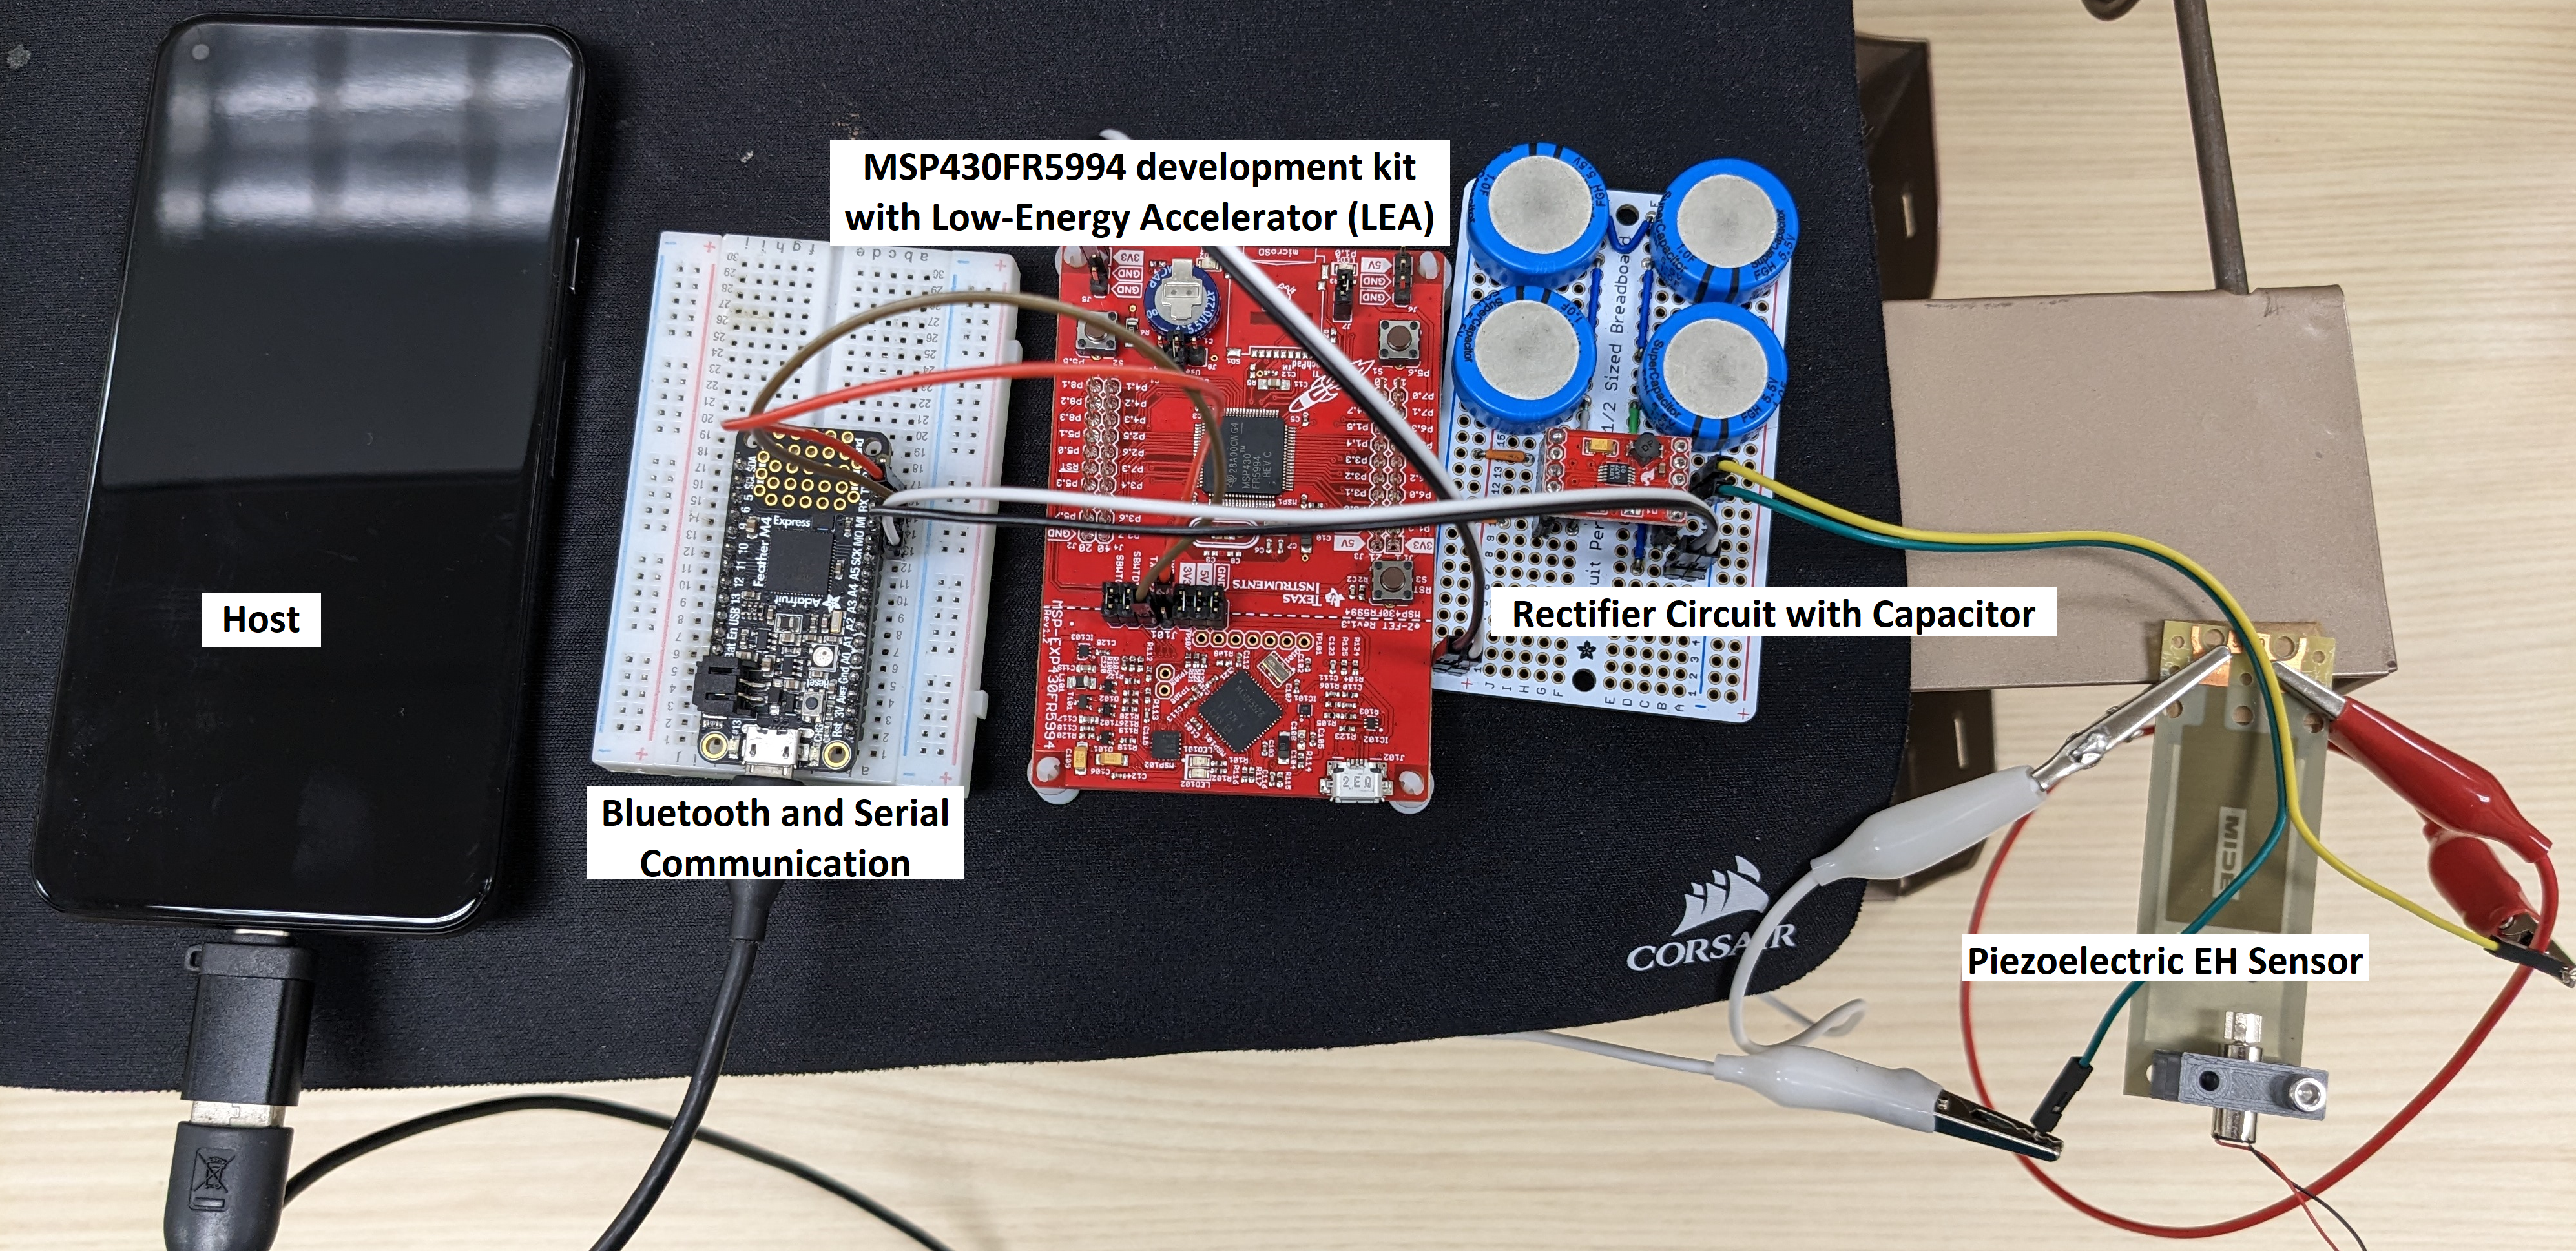
\includegraphics[clip, width=0.7\linewidth]{Chapter-4/IntermittentTrainingICLR25CameraReady/figs/SeekerCommercial.png}
  \caption{Hardware setup of NExUME using MSP-EXP430FR5994 as the edge compute, Adafruit ItsyBitsy nRF52840 Express for communicating, Energy Harvester Breakout - LTC3588 with supercapacitors as energy rectification and storage and a Pixel-5 phone as the host.}
  \label{Fig:cotsFIG}
\end{figure}

We use iNAS~\cite{intermittentNAS} to find the DNNs meeting the energy income and train them using our proposed DynFit. Table~\ref{tab:AccMSPonIND} shows the accuracy of classification tasks against the different baselines and state-of-the-art methods.

\begin{table}[ht]
\centering
\caption{Accuracy of NExUME and other methods for industry status monitoring dataset using TI MSP board and piezoelectric energy source. Results collected over 200 experiment cycles.}
\resizebox{\textwidth}{!}{%
\begin{tabular}{@{}ccccccccc@{}}
\toprule
\textbf{Class} & \textbf{Full Power} & \textbf{AP} & \textbf{PT} & \textbf{iNAS+PT} & \textbf{Stateful} & \textbf{ePerceptive} & \textbf{DynBal} & \textbf{NExUME} \\ \midrule
\textbf{R1}    & 84.93               & 74.46       & 77.02       & 79.62           & 80.85             & 81.50               & 82.15           & \textbf{83.60}  \\
\textbf{R2}    & 85.85               & 76.21       & 79.18       & 80.36           & 81.95             & 82.60               & 83.25           & \textbf{84.50}  \\
\textbf{R3}    & 81.09               & 72.43       & 75.38       & 78.18           & 79.05             & 79.70               & 80.35           & \textbf{80.85}  \\
\textbf{SJ}    & 90.95               & 82.33       & 85.00       & 87.58           & 88.60             & 89.15               & 89.80           & \textbf{90.50}  \\
\textbf{SI}    & 94.76               & 85.31       & 88.05       & 89.90           & 91.00             & 91.65               & 92.30           & \textbf{93.00}  \\ \bottomrule
\end{tabular}%
}
\label{tab:AccMSPonIND}
\end{table}

NExUME demonstrates superior performance across all operating classes, achieving the highest accuracy in each case. For example, for the spindle idle (SI) class, NExUME attains an accuracy of $93.00\%$, outperforming DynBal by $0.70\%$. While the margins may appear small, in industrial settings, even minor improvements in classification accuracy can have significant implications for predictive maintenance and operational efficiency.

The improved performance of NExUME in this real-world application further validates its effectiveness and practical utility. By effectively managing energy constraints and adapting to intermittent power conditions, NExUME enables more reliable and accurate monitoring in industrial environments where energy harvesting is a viable power solution.

\subsection{Sensitivity and Ablation Studies of NExUME}

To elucidate the influence of variable SLOs and hardware-specific settings on system performance, we conducted a comprehensive sensitivity study. This study involved adjusting the acceptable latency and the capacitance of the energy harvesting setup to assess their impacts on accuracy. As shown in Figure~\ref{Fig:accVlat}, the accuracy improves with increased latency, but with diminishing returns. Similarly, Figure~\ref{Fig:accVcap} demonstrates that, while increasing capacitance should theoretically stabilize the system, its charging characteristics can lead to extended charging times, thus exceeding the latency SLO. Notably, some anomalies in the data were attributed to abrupt power failures, a common challenge in intermittent energy harvesting systems.

\begin{figure}[ht]
\centering
\subfloat[Accuracy vs Latency]{
    \includegraphics[width=0.45\textwidth]{Chapter-4/IntermittentTrainingICLR25CameraReady/figs/ALcurve.pdf}
    \label{Fig:accVlat}
}
\subfloat[Accuracy vs Capacitance]{
    \includegraphics[width=0.45\textwidth]{Chapter-4/IntermittentTrainingICLR25CameraReady/figs/ACcurve.pdf}
    \label{Fig:accVcap}
}
\caption{Sensitivity analysis of NExUME showing the impact of (a) acceptable latency and (b) capacitance on accuracy across different platforms and energy sources.}
\label{Fig:sensitivity}
\end{figure}

An ablation study evaluates the contributions of individual components within NExUME. The results, plotted in Figure~\ref{Fig:abal}, indicate that the greatest improvements are derived from the synergistic operation of all components, particularly DynFit and DynInfer. Although iNAS enhances network selection, its lack of intermittency awareness significantly impacts accuracy.

\begin{figure}[ht]
\centering
\includegraphics[width=0.8\textwidth]{Chapter-4/IntermittentTrainingICLR25CameraReady/figs/ablationBW.pdf}
\caption{Ablation study showing the contribution of each component of NExUME to overall accuracy improvement across different datasets.}
\label{Fig:abal}
\end{figure}

The ablation results clearly demonstrate that the combination of all three components---DynNAS, DynFit, and DynInfer---yields the best performance. DynFit alone provides significant improvements by making the training process energy-aware, while DynInfer's scheduling optimizations are most effective when combined with a network that has been trained to handle intermittency.

\subsection{Performance on Different Hardware Platforms}

Our comprehensive evaluation across MSP430FR5994 and Arduino Nano 33 BLE demonstrates NExUME's platform independence. Figure~\ref{Fig:MSPRF} shows accuracy results on MSP with RF harvesting across different datasets, while Figure~\ref{Fig:ArduinoRF} presents corresponding results on Arduino.

\begin{figure}[ht]
\centering
\subfloat[MSP430FR5994 with RF]{
    \includegraphics[width=0.45\textwidth]{Chapter-4/IntermittentTrainingICLR25CameraReady/figs/MSPRF.pdf}
    \label{Fig:MSPRF}
}
\subfloat[Arduino Nano with RF]{
    \includegraphics[width=0.45\textwidth]{Chapter-4/IntermittentTrainingICLR25CameraReady/figs/ArduinoRF.pdf}
    \label{Fig:ArduinoRF}
}
\caption{Accuracy comparison across different datasets on (a) MSP430FR5994 and (b) Arduino Nano 33 BLE with RF energy harvesting.}
\label{Fig:platform_comparison}
\end{figure}

Similarly, piezoelectric harvesting results are shown in Figure~\ref{Fig:MSPPiezo} for MSP and Figure~\ref{Fig:ArduinoPiezo} for Arduino, while thermal harvesting results are presented in Figure~\ref{Fig:MSPThermal} and Figure~\ref{Fig:ArduinoThermal} respectively.

\begin{figure}[ht]
\centering
\subfloat[MSP with Piezoelectric]{
    \includegraphics[width=0.45\textwidth]{Chapter-4/IntermittentTrainingICLR25CameraReady/figs/MSPPiezo.pdf}
    \label{Fig:MSPPiezo}
}
\subfloat[Arduino with Piezoelectric]{
    \includegraphics[width=0.45\textwidth]{Chapter-4/IntermittentTrainingICLR25CameraReady/figs/ArduinoPiezo.pdf}
    \label{Fig:ArduinoPiezo}
}
\caption{Accuracy comparison on (a) MSP430FR5994 and (b) Arduino Nano with piezoelectric energy harvesting.}
\label{Fig:piezo_comparison}
\end{figure}

\begin{figure}[ht]
\centering
\subfloat[MSP with Thermal]{
    \includegraphics[width=0.45\textwidth]{Chapter-4/IntermittentTrainingICLR25CameraReady/figs/MSPThermal.pdf}
    \label{Fig:MSPThermal}
}
\subfloat[Arduino with Thermal]{
    \includegraphics[width=0.45\textwidth]{Chapter-4/IntermittentTrainingICLR25CameraReady/figs/ArduinoThermal.pdf}
    \label{Fig:ArduinoThermal}
}
\caption{Accuracy comparison on (a) MSP430FR5994 and (b) Arduino Nano with thermal energy harvesting.}
\label{Fig:thermal_comparison}
\end{figure}

Across all platforms and energy sources, NExUME consistently outperforms baselines with improvements ranging from $6\%$ to $22\%$, demonstrating the generality and robustness of our approach.

\section{Discussion and Future Directions}
\label{sec:nexume_discussion}

\subsection{Integration with Chapter 2 Systems}

The NExUME framework presented in this chapter naturally complements the distributed inference systems from Chapter~\ref{ch:intelligent-inference}. While Origin and Seeker focused on optimizing the distribution of inference tasks and minimizing communication costs in EH-WSNs, NExUME addresses the fundamental challenge of making individual DNNs aware of and adaptive to intermittent power conditions. The combination of these approaches creates a comprehensive solution where Origin/Seeker handles the system-level orchestration and communication optimization, while NExUME ensures that each individual node can effectively execute its assigned tasks despite power fluctuations.

Furthermore, the QuantaTask concept from NExUME could be integrated with Seeker's coreset-based compression to create atomic units of computation that are both energy-aware and communication-efficient. This would enable nodes to determine not only what to compute based on available energy, but also what compressed representation to transmit based on both energy and communication constraints.

\subsection{Theoretical Foundations}

While this work has demonstrated empirical success, several theoretical questions remain open. The convergence properties of DynFit under varying energy profiles need formal analysis. Specifically, we need to establish bounds on the training loss under different energy variability patterns and prove the stability of the adaptive regularization strategy. Additionally, the optimality gap of our scheduling heuristic needs tighter bounds, particularly for specific classes of task graphs commonly found in DNN inference.

The interaction between dropout rates, quantization levels, and energy availability creates a complex optimization landscape. Future work should explore whether there exist optimal policies for adjusting these parameters that can be computed efficiently, possibly through reinforcement learning or other adaptive control techniques.

\subsection{Hardware Acceleration Opportunities}

The success of NExUME opens several avenues for hardware acceleration. Custom accelerators could be designed specifically for QuantaTask execution, with built-in support for variable-precision computation and dynamic sparsity patterns induced by energy-aware dropout. ReRAM crossbar architectures, as mentioned in Chapter~\ref{ch:intelligent-inference}, could be enhanced with energy-monitoring circuits that directly inform the computation precision.

Figure~\ref{Fig:XBfull} shows a conceptual ReRAM crossbar accelerator that could be optimized for NExUME's dynamic computation requirements, while Figure~\ref{Fig:XBcell} illustrates the individual cell design that enables variable-precision operations.

\begin{figure}[ht]
\centering
\subfloat[Full Crossbar Architecture]{
    \includegraphics[width=0.45\textwidth]{Chapter-4/IntermittentTrainingICLR25CameraReady/figs/XBfull.png}
    \label{Fig:XBfull}
}
\subfloat[Cell-Level Design]{
    \includegraphics[width=0.45\textwidth]{Chapter-4/IntermittentTrainingICLR25CameraReady/figs/XBcell.png}
    \label{Fig:XBcell}
}
\caption{ReRAM crossbar accelerator concept for NExUME: (a) Full crossbar architecture supporting dynamic precision, (b) Individual cell design enabling variable-precision computation.}
\label{Fig:reram_concept}
\end{figure}

Furthermore, the predictive energy harvesting models used in DynInfer could be implemented in dedicated hardware predictors, similar to branch predictors in modern processors, to reduce the overhead of energy availability estimation.

\subsection{Broader Impact}

The implications of NExUME extend beyond energy harvesting systems. The principles of training DNNs to be aware of resource variability could be applied to other constrained environments, such as mobile devices with varying battery levels, cloud systems with dynamic pricing, or edge devices with fluctuating network connectivity. The framework challenges the traditional assumption that DNNs operate in stable resource environments and opens new research directions in adaptive machine learning.

\section{Conclusions}
\label{sec:nexume_conclusions}

This chapter presented NExUME, an advanced framework designed to optimize the training and inference phases of deep neural networks within the constraints of intermittently powered, energy-harvesting devices. By integrating adaptive neural architecture and energy-aware training techniques, NExUME significantly enhances the viability of deploying machine learning models in environments with limited and unreliable energy sources.

The results from our extensive evaluations demonstrate that NExUME can substantially outperform traditional methods in energy-constrained settings, with improvements in accuracy ranging from $6\%$ to $22\%$ over existing methods. These improvements highlight NExUME's capability to adapt dynamically to fluctuating energy conditions, ensuring both operational longevity and computational integrity.

The broader implication of this work extends beyond technological advancements, suggesting a paradigm shift in how the machine learning community approaches the design and deployment of systems in energy-limited environments. By prioritizing energy efficiency and system adaptability, NExUME contributes to the sustainability and accessibility of machine learning solutions, enabling their deployment in regions where power infrastructure is absent or unreliable. This is particularly crucial in developing regions where such technology can drive innovation in healthcare, agriculture, and education.

Furthermore, the development of energy-efficient, adaptive systems like NExUME is aligned with the growing need for sustainable computing practices across all disciplines of technology. It challenges the machine learning community to consider not only the accuracy and efficiency of algorithms but also their environmental impact and accessibility, ensuring a broader positive social impact.

Building on the distributed inference foundations from Chapter~\ref{ch:intelligent-inference} and setting the stage for the ultra-low power implementations in subsequent chapters, NExUME represents a critical advancement in making machine learning truly viable for the next generation of battery-free, sustainable computing systems. The next chapter will explore how these concepts can be pushed even further with specialized hardware architectures designed from the ground up for intermittent operation.